\chapter{Materiales y métodos}
En el presente capítulo se describen los materiales y métodos utilizados para el desarrollo, implementación y realización del proyecto. Se muestran por separado la parte hardware y la parte software. 

\section{Hardware}
En esta seccion \textbf{Hardware}, se definen y nombran los componentes hardware necesarios para la realización del proyecto, tanto los utilizados para el diseño y desarrollo como los correspondientes al dispositivo, que serán conectados en la placa principal, y que hacen posible que se cumplan las funciones que aporta cada uno de ellos al proyecto. Los elementos utilizados son los siguientes:

\begin{itemize}
	\item \textbf{Arduino MEGA 2560}
	\\
	Es el componente central del proyecto, se encarga de controlar al resto de elementos hardware que forman el sistema, así como de la ejecución del software.
	\begin{figure}[h]
    \centering
    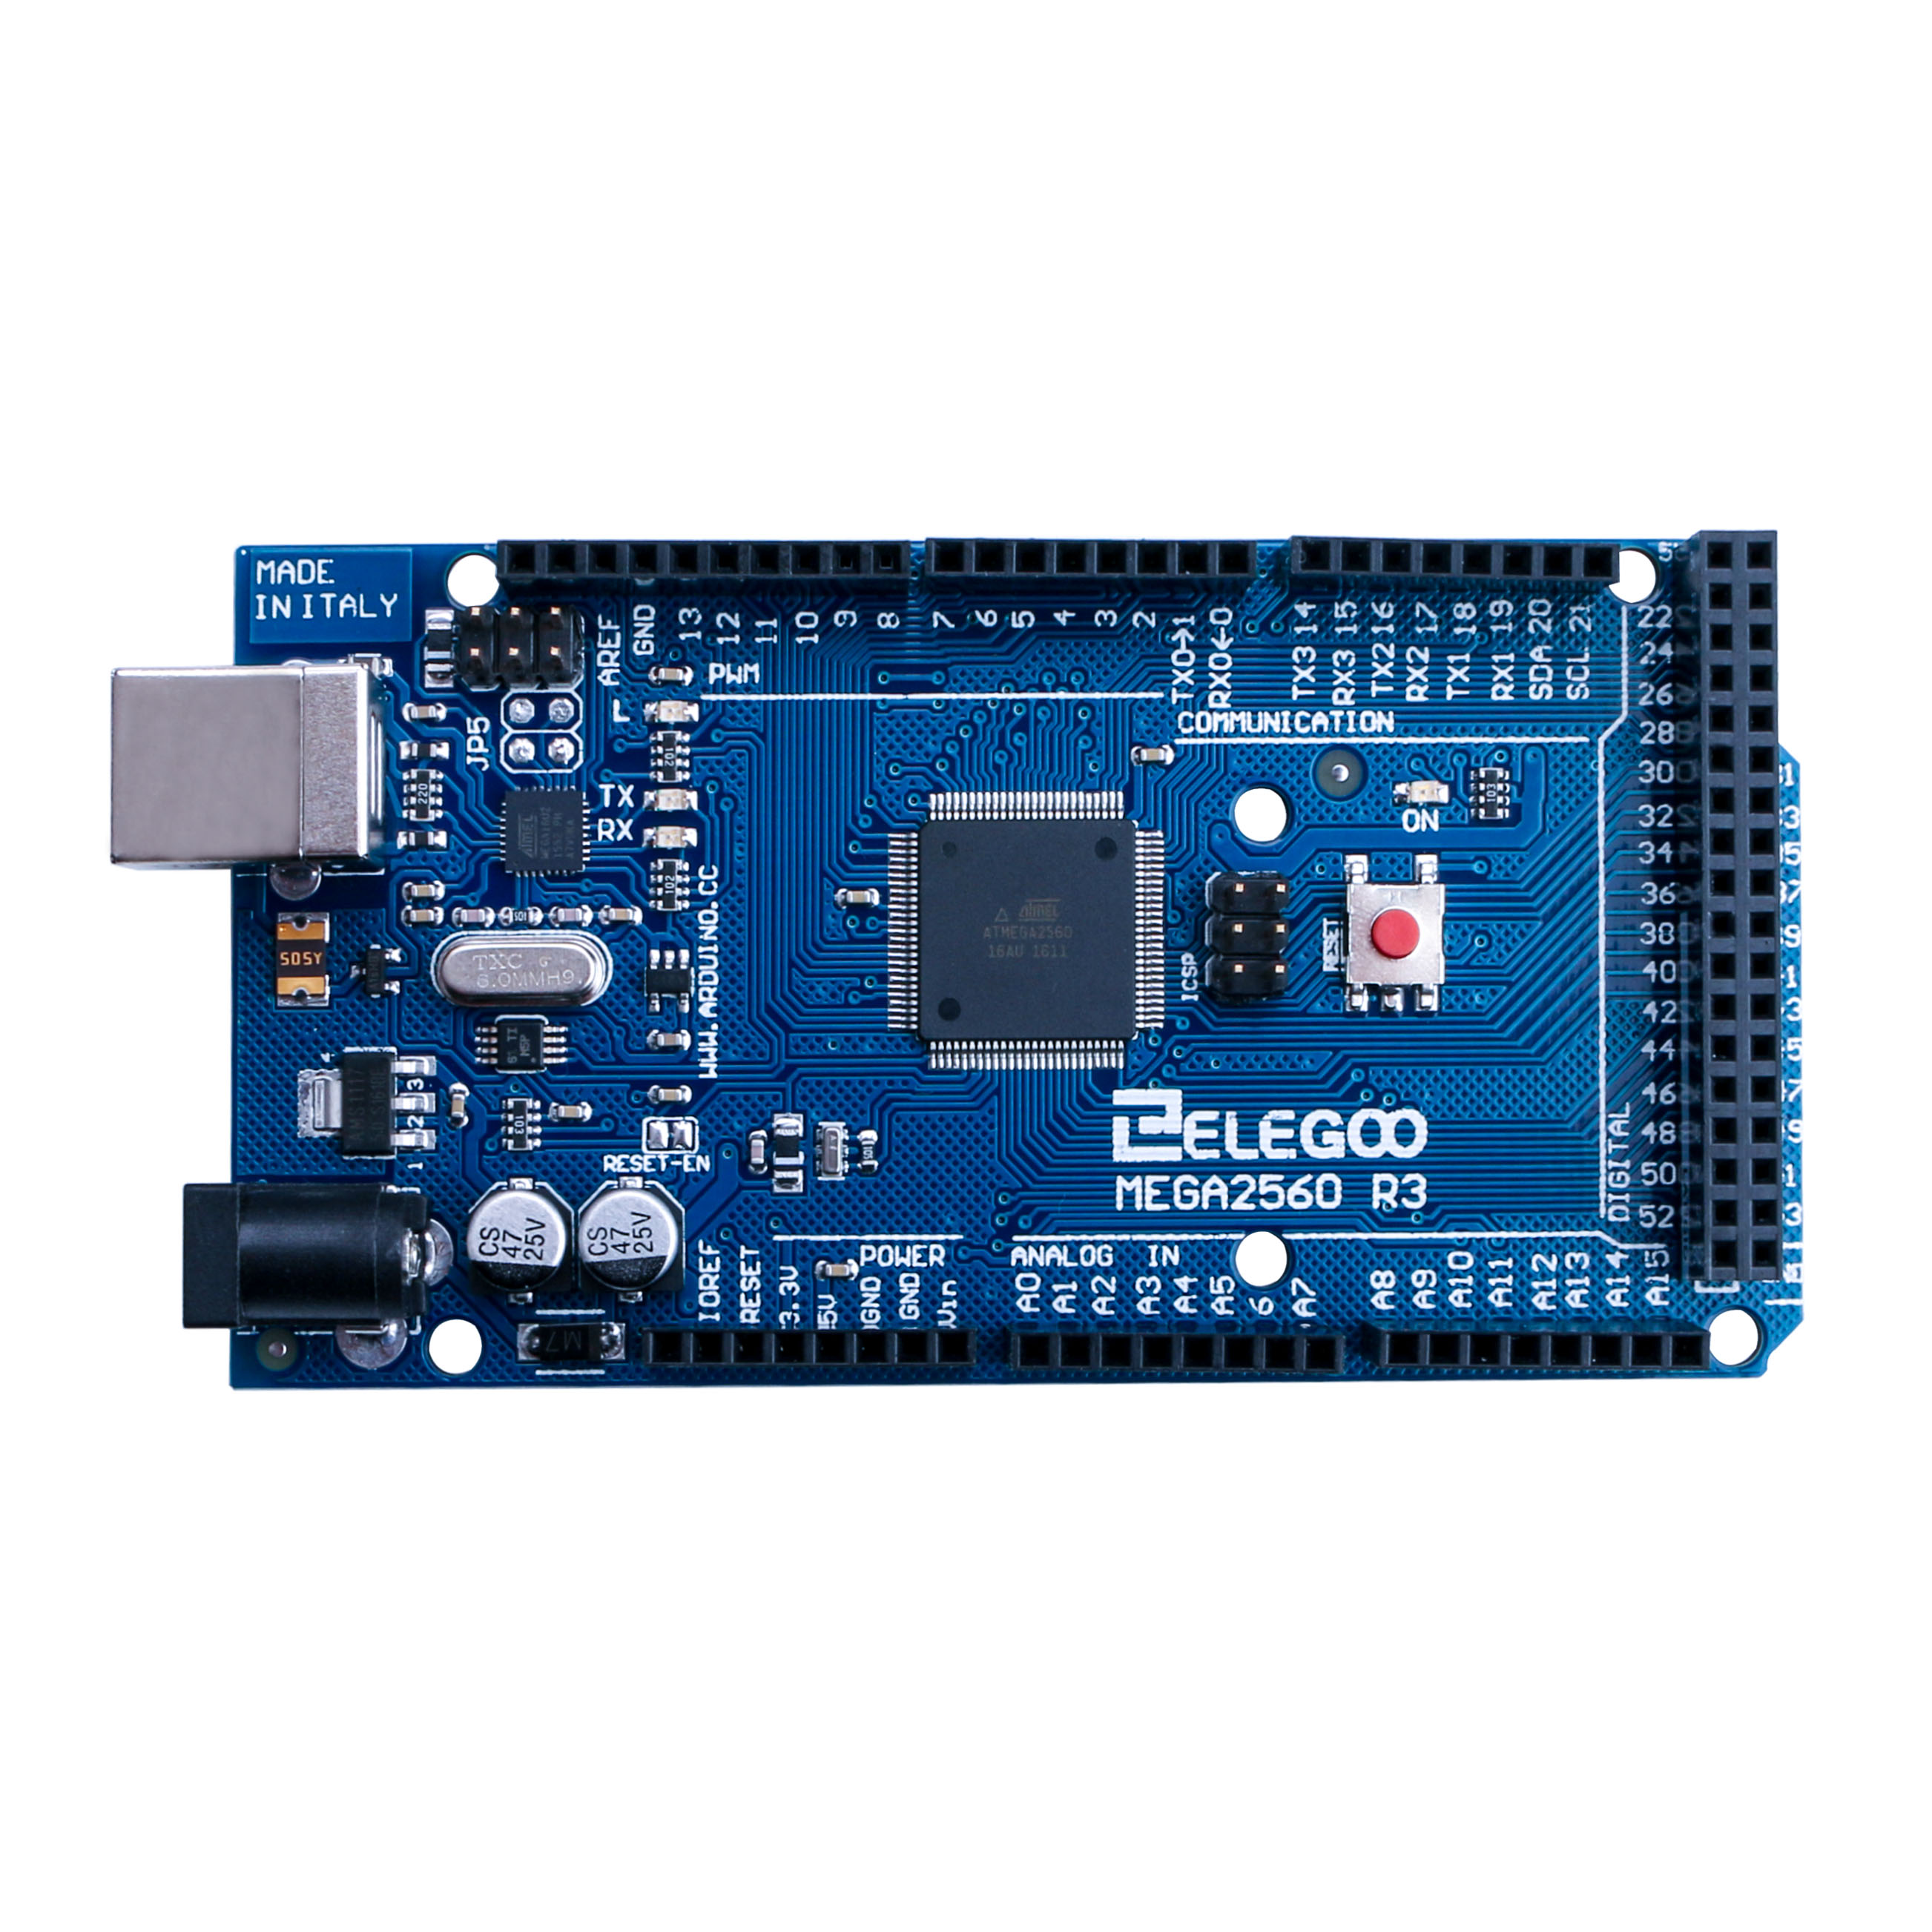
\includegraphics[width=0.4\textwidth]{imagenes/arduinomega.jpg}\\[1cm]
    \end{figure}
    
	\item \textbf{Pantalla LCD1602}
	\\
	Es el encargado de mostrar la visualización de la ejecución del programa principal, permitiendo de esta forma al usuario ser consciente en cada momento de las acciones que se están llevando a cabo en el sistema.
	\begin{figure}[h]
    \centering
    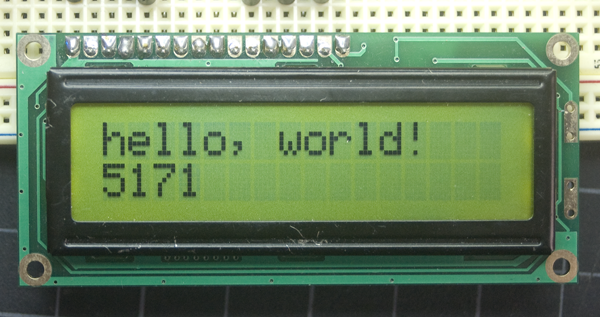
\includegraphics[width=0.4\textwidth]{imagenes/pantallalcd.png}\\[1cm]
    \end{figure}
    
	\item \textbf{Teclado matricial 4x4}
	\\
	Interfaz que actúa para ofrecer al usuario la capacidad de interactuar con la aplicación, para los juegos en dónde sea preciso su uso.
	\begin{figure}[h]
    \centering
    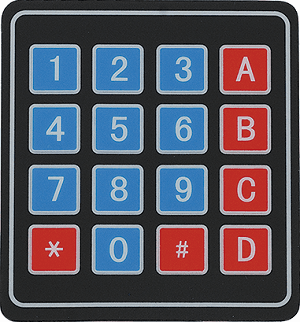
\includegraphics[width=0.3\textwidth]{imagenes/teclado4x4.png}\\[0.8cm]
    \end{figure}
    
	\item \textbf{Pulsadores de botón}
	\\
	Actúan también como interfaz entre el usuario y la aplicación, para los juegos dónde es necesario utilizarlos. 
	\item \textbf{Bombillas LED}
	\\
	Permiten la capacidad de ofrecer un estímulo visual al usuario para aumentar la capacidad de interacción entre este y la aplicación.
	
	\item \textbf{Resistencias y potenciómetro}
	\\
    Las resistencias son utilizadas para proteger diversos componentes del circuito y filtrar la corriente que circula por los elementos, evitando alteraciones o roturas por posibles subidas de tensión. El potenciómetro es necesario para controlar la tensión en la pantalla LCD y de esta forma conseguir el contraste óptimo para visualizar el contenido. 
\end{itemize}

\section{Software}
